\documentclass{article}
\usepackage{amsmath, amssymb}
\usepackage{bm}
\usepackage{graphicx} % Required for inserting images
\usepackage{tikz}
\usepackage{float}
\usepackage[round]{natbib}

\bibliographystyle{plainnat}
\usepackage[a4paper, top = 2cm,
                     bottom = 2cm,
                     left = 2cm,
                     right = 2cm]{geometry}


\title{Fences and baits : landscape connectivity in renewable resources}
\author{Simon Jean}
\date{July 2023}


%%%%%%%%%%%%%%%%%%%%%%
\newcommand*{\xMin}{0}%
\newcommand*{\xMax}{5}%
\newcommand*{\yMin}{0}%
\newcommand*{\yMax}{3}%


\newtheorem{assumption}{Assumption}

\begin{document}


\maketitle

\section{Motivation}
Assume I have a renewable resource whose habitat spans several land patches. The resource freely flows across patches according to some biological, exogenous determinants.  Assume we have 2 patches, A and B, such that the net benefit of harvest in A is larger than in B (people in A may love the resource, while in B they just like it; they may also be more efficient at harvesting it than in B). As people in A do love their resources, they may be tempted to ensure they stay in A and fence their land. They also notice that B has resources, and are tempted to increase the migration flow from B to A, and bait the resource into A. \\\\
The question that emerges is: how does the harvest of a renewable resource change when fencing and baiting are considered?

\section{Modeling strategy}
\subsection{A 2 patch model}
In each period and each patch, the resource stock $X_{At}$ and $ X_{Bt}$ is harvested at $h_{At}$ and $h_{Bt}$, leaving a remaining stock $e_{At}$ and $ e_{Bt}$ which then grows to $g_A(e_{At})$ and $g_B(e_{Bt})$, with $g'_i()>0$ and $g''_i()<0$. Once it grows, it migrates. For example, in patch $A$, a share $d_{AAt}$ of the stock remains in $A$ in period $t$, while a share $d_{ABt} = 1-d_{AAt}$ flows from $A$ to $B$, and reciprocally for $B$. At the beginning of period $t+1$ : 
\begin{align}
    X_{At+1} = (1-d_{ABt+1})g_A(e_{At})+d_{BAt}g_B(e_{Bt})
    \\
    X_{Bt+1} = (1 - d_{BAt+1})g_B(e_{BT}) + d_{ABt}g_A(e_{At})
\end{align}

In each period, after observing the dispersal flows, landowners choose whether to improve their fences, increase the baiting, or further improve their land. 
Dispersal in the next period will depend on each landowner's fencing $z_{At}^F$and $z_{Bt}^F$ and baiting and land improvement practices $z_{At}^B$ and $z_{Bt}^B$, as well as historical dispersal $d_{ABt}$, and natural, exogenous features that limit dispersal : 
\begin{align}
    d_{ABt+1} = f_{AB}(z^F_{At}, z^B_{Bt}| d_{ABt}) \in [m_{AB},M_{AB}] \subset [0,1] \\
    d_{BAt+1} = f_{BA}(z^F_{Bt}, z^B_{At}| d_{BAt}) \in [m_{BA},M_{BA}] \subset [0,1]
\end{align}
The more one landowner fences, the more it retains the resource. However, fencing is less and less effective at retaining the resources\footnote{It may be good to go back to this hypothesis: the effect of incomplete fencing may be concave, but convex at the end when the fence is finished}. Baiting increases the flow of dispersal from the neighboring patch at a decreasing rate as well. Baiting reduces the marginal effect of fencing and fencing reduces the marginal effect of baiting.

Eventually, future dispersal depends on existing dispersal $d_{ijt}$. The larger the existing dispersal, the larger the future dispersal, with a concave effect. Conditional on $d_{ijt}$, fencing has a positive yet decreasing effect on future dispersal, and baiting incrases the flow of dispersal from a patch to its neightbor at a decreasing rate. 


 Overall : 
\begin{align*}
    \frac{\partial f_{AB}}{\partial z^F_{At}}\leq 0 &\text{ and } \frac{\partial^2 f_{AB}}{\partial (z^F_{At})^2} \geq 0\\
    \frac{\partial f_{AB}}{\partial z^B_{Bt}}\geq 0 &\text{ and } \frac{\partial^2 f_{AB}}{\partial (z^B_{Bt})^2} \leq 0\\
    \frac{\partial ^2 f_{AB}}{\partial z_{Bt}^B\partial z_{At}^F} \leq 0 &\text{ and } \frac{\partial ^2 f_{AB}}{\partial z_{At}^F\partial z_{Bt}^B} \leq 0
\end{align*}
\textbf{Add derivatives wrt to $d_{abt}$}


The timing of the model is synthetized in figure \ref{fig:timing}.

\begin{figure}[H]
  \centering
  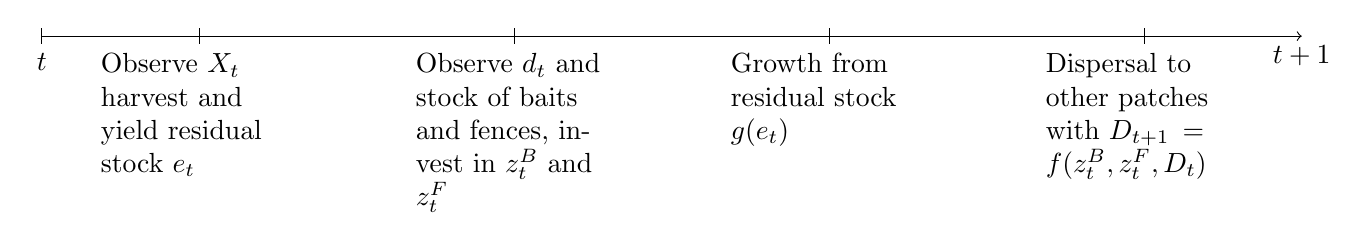
\begin{tikzpicture}
    % Draw the arrow
    \draw[->] (0,0) -- (16,0) node[anchor=north] {$t+1$};
    % Draw ticks and labels
    \draw (0, .1)--(0,-.1) node[anchor = north]{$t$};
    \draw (2, .1)--(2,-.1) node[anchor = north, text width = 2.5cm]{Observe $X_t$ harvest and yield residual stock $e_t$};
    \draw (6, .1)--(6,-.1) node[anchor = north, text width = 2.5cm] {Observe $d_t$ and stock of baits and fences, invest in $z_t^B$ and $z_t^F$};
    \draw (10, .1)--(10,-.1) node[anchor = north, text width = 2.5cm]{Growth from residual stock $g(e_t)$};
    \draw (14,.1)--(14,-.1) node[anchor = north, text width = 2.5cm]{Dispersal to other patches with $D_{t+1}=f(z_t^B, z_t^F, D_t)$};
  \end{tikzpicture}
  \caption{Timing of the model}
  \label{fig:timing}
\end{figure}

\subsection{Model formulation}
Landowners locally harvest the resource at a \textit{constant unit marginal cost} $\omega_i$ and sell it on a competitive market at price $p$, so the net marginal benefit is heterogeneous and can be written as $p_i = p - c_i$. Moreover, they choose fencing and baiting expenditures with costs $c_{i,l}(z_{it}^F)$ such that $c'_{i,l}\geq 0$ and $c''_{i,l} \geq 0$, and normalized such that $c_{i,l}(0) = 0$. The profit flow at time $t$ is
\begin{equation}
    \Pi_{it} = p_i(X_{it} - e_{it}) - c_{i,F}(z_{it}^F) - c_{i,B}(z_{it}^B)
\end{equation}

First, I'm interested in the social planner's problem, i.e, to maximize the intertemporal sum of discounted profits:
\begin{align*}
    \max_{\{e_{it}, z_{it}^F, z_{it}^B \}_{i \in \{A,B\}}} & \sum_{t=0}^T \delta^t \left( \sum_{i \in \{A,B\}} p_i(X_{it} - e_{it}) - c_{iF}(z_{it}^F) - c_{iB}(z_{it}^B) \right)\\
     &\text{Such that:}\\
        X_{At+1} &= (1-d_{ABt+1})g_A(e_{At})+d_{BAt}g_B(e_{Bt})
    \\
    X_{Bt+1} &= (1 - d_{BAt+1})g_B(e_{BT}) + d_{ABt}g_A(e_{At})\\
     d_{ABt+1} &= f_{AB}(z^F_{At}, z^B_{Bt}| d_{ABt}) \\
    d_{BAt+1} &= f_{BA}(z^F_{Bt}, z^B_{At}| d_{BAt})
\end{align*}
\section{Model resolution and insights}
First, due to the recursive nature of the problem, if a solution exists, we can write the Bellman equation : 

\begin{equation}
    V_t(\mathbf{X}_t, \mathbf{D}_t) = \max_{\{e_{it}, z_{it}^F, z_{it}^B\}_{i \in \{A,B\}}} \sum_{i \in \{A,B\}} p_i(X_{it} - e_{it}) - c_{iF}(z_{it}^F) - c_{iB}(z_{it}^B) + \delta V_{t+1}(\mathbf{X}_{t+1}, \mathbf{D}_{t+1})
\end{equation}
\subsection{Using backward induction}
As $T$ is the end of the planning horizon, any resource left over in $T+1$ will have no value. Therefore, the optimal policies in $T$ are to exhaust the existing stocks, and not to invest in connectivity, i.e $e_{AT}=e_{BT}=z_{AT}^F = z_{AT}^B = z_{BT}^F = z_{BT}^B=0$, and the value function in $T$ is :
$$
V_T(\mathbf{X}_T, \mathbf{D}_T) = p_A X_{AT} + p_B X_{BT}
$$

Therefore, in $T-1$:
\begin{align*}
    V_{T-1}(\mathbf{X}_{T-1}, \mathbf{D}_{T-1}) = \max_{\{e_{iT-1}, z_{iT-1}^F, z_{iT-1}^B \}_{i \in \{A,B\}}} \sum_{i \in \{A,B\}} & p_i(X_{iT-1} - e_{iT-1}) - c_{iF}(z_{iT-1}^F) - c_{iB}(z_{iT-1}^B) \\&+ \delta (p_A X_{AT} + p_B X_{BT})
\end{align*}
Using the laws of motion of dispersal and the resource, I get the following first-order conditions for interior solutions of $\{e_{AT-1}, e_{BT-1}, z_{AT-1}^F, z_{AT-1}^B, z_{BT-1}^F, z_{BT-1}^B\}$:
\begin{align}
    \frac{\partial V_{T-1}}{\partial e_{AT-1}} = 0 &\Rightarrow g'_A(e_{AT-1}) = \frac{p_A}{\delta (p_A (1-f_{AB}(z_{AT-1}^F, z_{BT-1}^B, d_{ABt}))+ p_B f_{AB}(z_{AT-1}^F, z_{BT-1}^B, d_{ABt}))} \label{eq:foc_e}\\
    \frac{\partial V_{T-1}}{\partial z_{AT-1}^B} = 0 &\Rightarrow c'_{AB}(z_{AT-1}^B) = \delta (p_A - p_B) g_B(e_{BT-1} )\frac{\partial f_{BA}}{\partial z_{AT-1}^B} \label{eq:foc_baiting}\\
    \frac{\partial V_{T-1}}{\partial z_{AT-1}^F} = 0 &\Rightarrow c'_{AF}(z_{AT-1}^F) = \delta (p_B - p_A) g_A(e_{AT-1} )\frac{\partial f_{AB}}{\partial z_{AT-1}^F} \label{eq:foc_fencing}
\end{align}
And the same sort of expression holds for $B$. \\\\
\subsubsection{Economic intuition from first order conditions}
First, equation \ref{eq:foc_e} is reminiscent of \cite{costello_optimal_2008}, and carries the same sort of intuition with time invariant exogenous dispersal: taking into account dispersal, the stock in patch $i$ must be harvested down to the point where the current forgone revenue of not harvesting one more unit ($p_A$) equals the future discounted benefit from additional growth ($g'_A(e_{AT-1})$) that disperses to patches where it is sold in the next period, hence the discount ($\delta (p_A (1-f_{AB}(z_{AT-1}^F, z_{BT-1}^B, d_{ABt}))+ p_B f_{AB}(z_{AT-1}^F, z_{BT-1}^B, d_{ABt}))$.
\\\\
Equation \ref{eq:foc_baiting} carries some interesting properties: for positive baiting to be an optimal strategy (i.e. $c'_{AB}()>0$), it must be that the resource is more valuable in $A$ than in $B$. In this set-up, the value component of the marginal benefit (i.e. $\delta (p_A - p_B)$) is independent of baiting, but the volume component changes with baiting (i.e $g_B(e_{BT-1})\frac{\partial f_{BA}}{\partial z_{AT-1}^B}$). Equation \ref{eq:foc_fencing} shows that, for some positive fencing to occur, the value of the resource must be larger in $A$ than in $B$ as well.

\subsubsection{Properties of the solution}
Harvesting, fencing and baiting are jointly determined. Using equation \ref{eq:foc_e}, one can define $e_{iT-1}=\Phi_i(z_{AT-1}^F, z_{BT-1}^B)$, with $\Phi_i = g'^{(-1)}_i(RHS)$, and $RHS$ the right-hand side of equation (15). In the end, a general (?) solution may emerge from a 4 equations system.

While $\mathbf{X}_{t+1} = \mathbf{D}_{t+1}g(\mathbf{e_t})$, it seems that the optimal policy functions can be time independent. Consider the case where fences and baits totally deplete between each period, such that they are flow variables but merely form stock. In this case, $f_{ij}(z_{it}^F, z_{jt}^B, d_{ijt})\equiv f_{ij}(z_{it}^F, z_{jt}^B, d_{ij})$, dispersal only depends on current decisions and exogenous parameters, then the choice of $e_t$ itself seems to be state independent. However, if fences and baits, or land improvement, do not fully decay and do form some stock, influencing the dispersal, it seems like the solution does not display state independence. 

Although solutions depend on parametric assumptions, the results concerning fencing and baiting imply corner solutions. In the optimum, the condition for fencing or baiting to be positive imply a binary ordering of prices in each patch. If $p_A>p_B$, investing in fencing and baiting to keep and drag the resource in its most valuable market makes sense. Investment in connectivity devices maximizes the arbitrage opportunity between the two patches. The amount of investment equates the marginal cost with the discounted additional benefit from changing the dispersal of the resource, or is constrained by natural exogenous parameters. If the marginal cost is low, and there are no natural exogenous bounds to dispersal between patches, then patch $A$ would attract all resources. It remains unclear if the harvesting rule changes.\\
From the corner solution that necessarily emerges, if $f_{AB}(z_{At}^F,0, d_{ABt})$ is additively separable in $d_{ijt}$ i.e $f_{AB}(z_{it}^F,0, d_{ABt}) \equiv \Psi_{AB}\left(\mu(z_{At}^F) + d_{ABt}\right)$ with $\Psi_{AB}()$ and $\mu()$ invertible,  it is possible to express the investment choices as a function of the state variables alone and to leverage the Dynamic Envelope Theorem.
\\\\
Overall, the optimal equilibrium maximizes the arbitrage opportunities between the two patches, and is constrained by the marginal cost function or the natural exogenous boundaries to dispersal. In the case where the marginal benefit would be decreasing and change sign, the optimal solution would still yield corner solutions, but would result in the absence of arbitrage opportunities\\
It seems that investing in dispersal is akin to installing a market between producers with costly transactions, where the transaction cost increases as the marginal cost adjusted by the productivity of investing in connectivity. 

\subsection{A perfect foresight analysis using the Dynamic Envelope Theorem}
Assume the land planner knows that the net marginal benefit is (i) time independent, and (ii) always larger in $A$ than in $B$ i.e. $\forall t, p_{At}=p_A \geq p_B$. In this case, it is clear that $z_{Bt}^F=z_{Bt}^B=0$. \\


In this case, assuming additive separability of $f$, that is to say
$ f(z_t^F, 0|d_t) \equiv f \left(  \psi (z_t^F) + \mu (d_{ABt} ) \right) $ where $f$ is increasing and concave and bounded above and below. $\psi$ is the production function mapping investment to dispersal and $\mu$ maps the historical dependence. 
\begin{align*}
d_{ABt+1} = f_{AB}(z_{At}^F, 0| d_{ABt}) & \Rightarrow z_{At}^F = \psi_{AB}^{-1}\left( f_{AB}^{(-1)}(d_{ABt+1}) - \mu(d_{ABt})\right) \\
d_{BAt+1} = f_{AB}(0, z_{At}^B| d_{ABt})& \Rightarrow z_{At}^B =\psi_{BA}^{-1} \left( f_{BA}^{(-1)}(d_{BAt+1}) - \mu(d_{BAt}) \right)\\
\end{align*}
Additionally, I think I can express $\mathbf{e}_t$ as a function of $\mathbf{X}_t, \mathbf{X}_{t+1}$ and $\mathbf{D}_t$.

\begin{enumerate}
	\item $z_t$ can be framed as $\Psi_{ij}(d_{ijt+1}; d_{ijt})$ with $\Psi$ increasing in its first argument and decreasing in its second. The question is how the second derivatives behave, which remains to be seen
	\item I'm not sure this works with inverting $e_t$ with $\mathbf{X_{t+1}, X_t, D_{t+1}}$...
\end{enumerate}

Use the framing for the interior solution and derivate around the optimum? \\


\subsection{A recurrence solution in an infinite horizon}
In this section, I explore the value function at any given point $t$ in time such that $t<T-1$, when the planning horizon is extended towards $T \to \infty$.
\\\\
For interior solutions to exist for $\{e_{At}, e_{Bt}, z_{At}^F, z_{At}^B, z_{Bt}^F, z_{Bt}^B\}$, it must be that : 

\begin{align*}
	V_t(\mathbf{D}_t, \mathbf{X}_t) &= \max_{\{e_{iT-1}, z_{iT-1}^F, z_{iT-1}^B \}_{i \in \{A,B\}}} \sum_{i \in \{A,B\}} p_i(X_{iT-1} - e_{iT-1}) - c_{iF}(z_{iT-1}^F) - c_{iB}(z_{iT-1}^B) + \delta V_{t+1}(\mathbf{D}_{t+1},\mathbf{X}_{t+1})\\
%
				  &= \max_{\{e_{iT-1}, z_{iT-1}^F, z_{iT-1}^B \}_{i \in \{A,B\}}} \sum_{i \in \{A,B\}} p_i(X_{iT-1} - e_{iT-1}) - c_{iF}(z_{iT-1}^F) - c_{iB}(z_{iT-1}^B) + \delta V_{t+1}(\mathbf{X}_{t+1}(\mathbf{e}_t, \mathbf{D}_{t+1}))\\
%
&= \max_{\{e_{iT-1}, z_{iT-1}^F, z_{iT-1}^B \}_{i \in \{A,B\}}} \sum_{i \in \{A,B\}}  p_i(X_{iT-1} - e_{iT-1}) - c_{iF}(z_{iT-1}^F) - c_{iB}(z_{iT-1}^B) \\
& + \delta V_{t+1}((1-d_{ABt+1})g_A(e_{At})+d_{BAt}g_B(e_{Bt});(1 - d_{BAt+1})g_B(e_{BT}) + d_{ABt}g_A(e_{At}))
\end{align*}
Where the second line outlines the dependence of future stocks on the remaining stock and the dispersal resulting from fencing and baiting choices. 

For an interior solution to emerge, the solution will not be state independent. To see this, see the FOCs that must hold for interior solutions to exist:


\section{Where I need help}
First, I need to fix things when it comes to the link between expenditures in fencing and baiting and how it relates to the dispersal, to maybe come closer to a dynamic envelope theorem solution. \\
Maybe one of the ways to do that is to clarify the equations in terms of units : in what I had in mind, for example using the sigmoid function : 
$$
d_{ABt+1} = m_{AB} + \frac{M_{AB} - m_{AB}}{1+ \exp(-(z_{At}^F + \beta d_{ABt}))}
$$
There is an incoherence : one flow is measured in \$, the other is unitless. It makes no sense to have a fraction exogenously decreasing; what might make sense is to consider the link between the current and historical flows, and see if there is decay in the quantity of fences or baits. I want to avoid as much as possible a convoluted approach, so maybe take some time to \textit{think of an approach that (i) encompasses the general conditions, clarifies the link (ii) between investment, capital and dispersal, and also (iii) check if it makes some sense??}.\\


Second, I need to conclude on the link between harvesting and investing, the link between the two is difficult to assess. \\\\

Third, is it really about fencing and baiting? What are the main things that economic geography has developed, that need to be studied in an environmental econ perspective? \\\\

Fourth, how can I make this more empirically relevant? 
\\\\
Fifth, how does this relate to wildfire spread and defensive investment? Is it already baked within the model? Can $d_{abt}$ be viewed as a spread probability conditional on ignition? Maybe in this case, $d$ would depend on existing stock, and \textit{next period} stock would also depend on $d$.


\newpage
\bibliography{resources}
\end{document}
